\documentclass[1p]{elsarticle_modified}
%\bibliographystyle{elsarticle-num}

%\usepackage[colorlinks]{hyperref}
%\usepackage{abbrmath_seonhwa} %\Abb, \Ascr, \Acal ,\Abf, \Afrak
\usepackage{amsfonts}
\usepackage{amssymb}
\usepackage{amsmath}
\usepackage{amsthm}
\usepackage{scalefnt}
\usepackage{amsbsy}
\usepackage{kotex}
\usepackage{caption}
\usepackage{subfig}
\usepackage{color}
\usepackage{graphicx}
\usepackage{xcolor} %% white, black, red, green, blue, cyan, magenta, yellow
\usepackage{float}
\usepackage{setspace}
\usepackage{hyperref}

\usepackage{tikz}
\usetikzlibrary{arrows}

\usepackage{multirow}
\usepackage{array} % fixed length table
\usepackage{hhline}

%%%%%%%%%%%%%%%%%%%%%
\makeatletter
\renewcommand*\env@matrix[1][\arraystretch]{%
	\edef\arraystretch{#1}%
	\hskip -\arraycolsep
	\let\@ifnextchar\new@ifnextchar
	\array{*\c@MaxMatrixCols c}}
\makeatother %https://tex.stackexchange.com/questions/14071/how-can-i-increase-the-line-spacing-in-a-matrix
%%%%%%%%%%%%%%%

\usepackage[normalem]{ulem}

\newcommand{\msout}[1]{\ifmmode\text{\sout{\ensuremath{#1}}}\else\sout{#1}\fi}
%SOURCE: \msout is \stkout macro in https://tex.stackexchange.com/questions/20609/strikeout-in-math-mode

\newcommand{\cancel}[1]{
	\ifmmode
	{\color{red}\msout{#1}}
	\else
	{\color{red}\sout{#1}}
	\fi
}

\newcommand{\add}[1]{
	{\color{blue}\uwave{#1}}
}

\newcommand{\replace}[2]{
	\ifmmode
	{\color{red}\msout{#1}}{\color{blue}\uwave{#2}}
	\else
	{\color{red}\sout{#1}}{\color{blue}\uwave{#2}}
	\fi
}

\newcommand{\Sol}{\mathcal{S}} %segment
\newcommand{\D}{D} %diagram
\newcommand{\A}{\mathcal{A}} %arc


%%%%%%%%%%%%%%%%%%%%%%%%%%%%%5 test

\def\sl{\operatorname{\textup{SL}}(2,\Cbb)}
\def\psl{\operatorname{\textup{PSL}}(2,\Cbb)}
\def\quan{\mkern 1mu \triangleright \mkern 1mu}

\theoremstyle{definition}
\newtheorem{thm}{Theorem}[section]
\newtheorem{prop}[thm]{Proposition}
\newtheorem{lem}[thm]{Lemma}
\newtheorem{ques}[thm]{Question}
\newtheorem{cor}[thm]{Corollary}
\newtheorem{defn}[thm]{Definition}
\newtheorem{exam}[thm]{Example}
\newtheorem{rmk}[thm]{Remark}
\newtheorem{alg}[thm]{Algorithm}

\newcommand{\I}{\sqrt{-1}}
\begin{document}

%\begin{frontmatter}
%
%\title{Boundary parabolic representations of knots up to 8 crossings}
%
%%% Group authors per affiliation:
%\author{Yunhi Cho} 
%\address{Department of Mathematics, University of Seoul, Seoul, Korea}
%\ead{yhcho@uos.ac.kr}
%
%
%\author{Seonhwa Kim} %\fnref{s_kim}}
%\address{Center for Geometry and Physics, Institute for Basic Science, Pohang, 37673, Korea}
%\ead{ryeona17@ibs.re.kr}
%
%\author{Hyuk Kim}
%\address{Department of Mathematical Sciences, Seoul National University, Seoul 08826, Korea}
%\ead{hyukkim@snu.ac.kr}
%
%\author{Seokbeom Yoon}
%\address{Department of Mathematical Sciences, Seoul National University, Seoul, 08826,  Korea}
%\ead{sbyoon15@snu.ac.kr}
%
%\begin{abstract}
%We find all boundary parabolic representation of knots up to 8 crossings.
%
%\end{abstract}
%\begin{keyword}
%    \MSC[2010] 57M25 
%\end{keyword}
%
%\end{frontmatter}

%\linenumbers
%\tableofcontents
%
\newcommand\colored[1]{\textcolor{white}{\rule[-0.35ex]{0.8em}{1.4ex}}\kern-0.8em\color{red} #1}%
%\newcommand\colored[1]{\textcolor{white}{ #1}\kern-2.17ex	\textcolor{white}{ #1}\kern-1.81ex	\textcolor{white}{ #1}\kern-2.15ex\color{red}#1	}

{\Large $\underline{12n_{0756}~(K12n_{0756})}$}

\setlength{\tabcolsep}{10pt}
\renewcommand{\arraystretch}{1.6}
\vspace{1cm}\begin{tabular}{m{100pt}>{\centering\arraybackslash}m{274pt}}
\multirow{5}{120pt}{
	\centering
	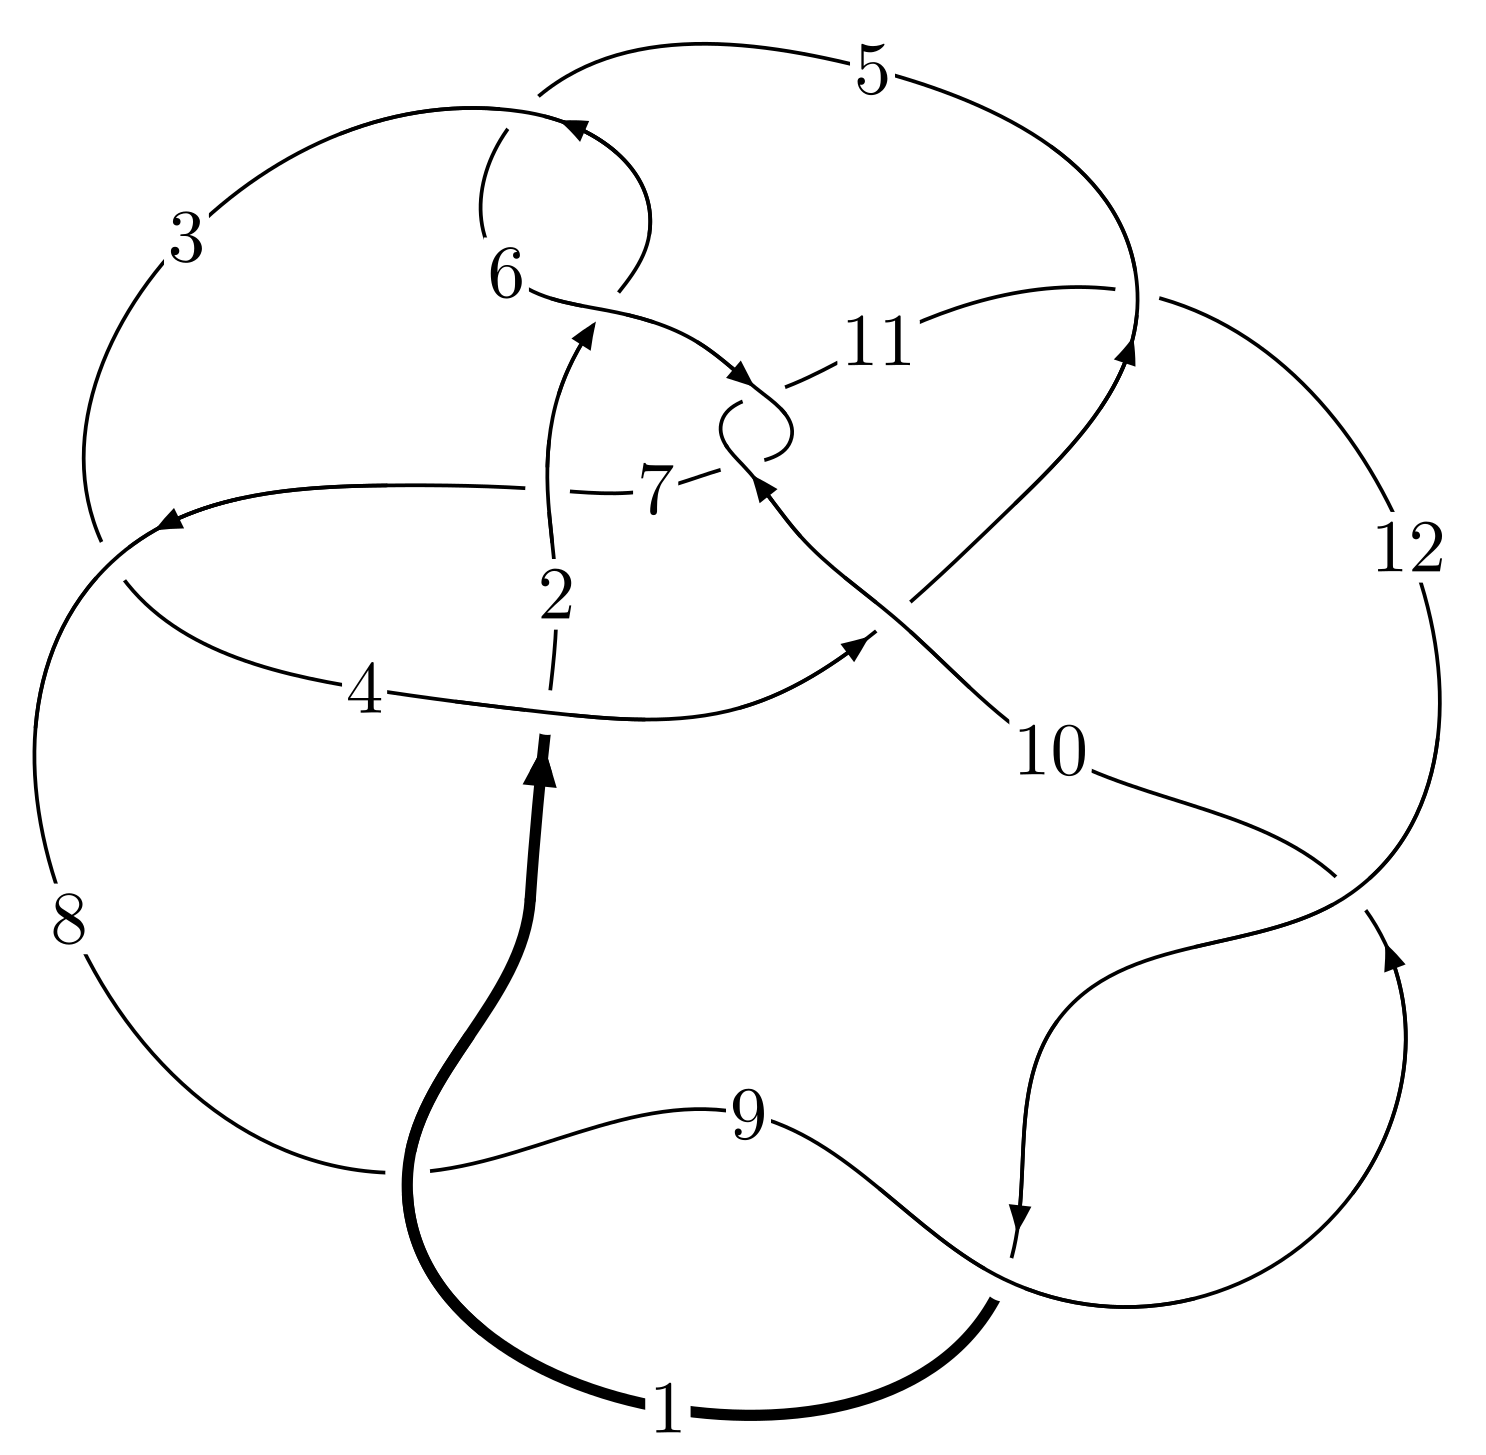
\includegraphics[width=112pt]{../../../GIT/diagram.site/Diagrams/png/2845_12n_0756.png}\\
\ \ \ A knot diagram\footnotemark}&
\allowdisplaybreaks
\textbf{Linearized knot diagam} \\
\cline{2-2}
 &
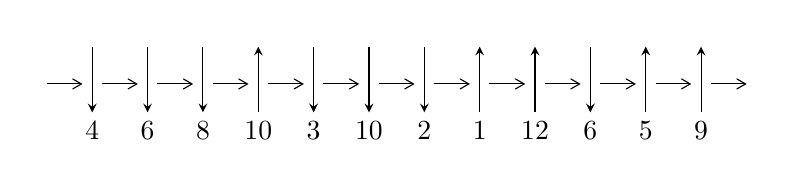
\begin{tikzpicture}[x=20pt, y=17pt]
	% nodes
	\node (C0) at (0, 0) {};
	\node (C1) at (1, 0) {};
	\node (C1U) at (1, +1) {};
	\node (C1D) at (1, -1) {4};

	\node (C2) at (2, 0) {};
	\node (C2U) at (2, +1) {};
	\node (C2D) at (2, -1) {6};

	\node (C3) at (3, 0) {};
	\node (C3U) at (3, +1) {};
	\node (C3D) at (3, -1) {8};

	\node (C4) at (4, 0) {};
	\node (C4U) at (4, +1) {};
	\node (C4D) at (4, -1) {10};

	\node (C5) at (5, 0) {};
	\node (C5U) at (5, +1) {};
	\node (C5D) at (5, -1) {3};

	\node (C6) at (6, 0) {};
	\node (C6U) at (6, +1) {};
	\node (C6D) at (6, -1) {10};

	\node (C7) at (7, 0) {};
	\node (C7U) at (7, +1) {};
	\node (C7D) at (7, -1) {2};

	\node (C8) at (8, 0) {};
	\node (C8U) at (8, +1) {};
	\node (C8D) at (8, -1) {1};

	\node (C9) at (9, 0) {};
	\node (C9U) at (9, +1) {};
	\node (C9D) at (9, -1) {12};

	\node (C10) at (10, 0) {};
	\node (C10U) at (10, +1) {};
	\node (C10D) at (10, -1) {6};

	\node (C11) at (11, 0) {};
	\node (C11U) at (11, +1) {};
	\node (C11D) at (11, -1) {5};

	\node (C12) at (12, 0) {};
	\node (C12U) at (12, +1) {};
	\node (C12D) at (12, -1) {9};
	\node (C13) at (13, 0) {};

	% arrows
	\draw[->,>={angle 60}]
	(C0) edge (C1) (C1) edge (C2) (C2) edge (C3) (C3) edge (C4) (C4) edge (C5) (C5) edge (C6) (C6) edge (C7) (C7) edge (C8) (C8) edge (C9) (C9) edge (C10) (C10) edge (C11) (C11) edge (C12) (C12) edge (C13) ;	\draw[->,>=stealth]
	(C1U) edge (C1D) (C2U) edge (C2D) (C3U) edge (C3D) (C4D) edge (C4U) (C5U) edge (C5D) (C6U) edge (C6D) (C7U) edge (C7D) (C8D) edge (C8U) (C9D) edge (C9U) (C10U) edge (C10D) (C11D) edge (C11U) (C12D) edge (C12U) ;
	\end{tikzpicture} \\
\hhline{~~} \\& 
\textbf{Solving Sequence} \\ \cline{2-2} 
 &
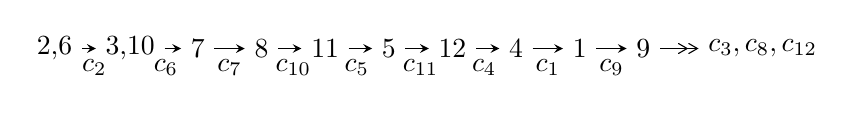
\begin{tikzpicture}[x=23pt, y=7pt]
	% node
	\node (A0) at (-1/8, 0) {2,6};
	\node (A1) at (17/16, 0) {3,10};
	\node (A2) at (17/8, 0) {7};
	\node (A3) at (25/8, 0) {8};
	\node (A4) at (33/8, 0) {11};
	\node (A5) at (41/8, 0) {5};
	\node (A6) at (49/8, 0) {12};
	\node (A7) at (57/8, 0) {4};
	\node (A8) at (65/8, 0) {1};
	\node (A9) at (73/8, 0) {9};
	\node (C1) at (1/2, -1) {$c_{2}$};
	\node (C2) at (13/8, -1) {$c_{6}$};
	\node (C3) at (21/8, -1) {$c_{7}$};
	\node (C4) at (29/8, -1) {$c_{10}$};
	\node (C5) at (37/8, -1) {$c_{5}$};
	\node (C6) at (45/8, -1) {$c_{11}$};
	\node (C7) at (53/8, -1) {$c_{4}$};
	\node (C8) at (61/8, -1) {$c_{1}$};
	\node (C9) at (69/8, -1) {$c_{9}$};
	\node (A10) at (11, 0) {$c_{3},c_{8},c_{12}$};

	% edge
	\draw[->,>=stealth]	
	(A0) edge (A1) (A1) edge (A2) (A2) edge (A3) (A3) edge (A4) (A4) edge (A5) (A5) edge (A6) (A6) edge (A7) (A7) edge (A8) (A8) edge (A9) ;
	\draw[->>,>={angle 60}]	
	(A9) edge (A10);
\end{tikzpicture} \\ 

\end{tabular} \\

\footnotetext{
The image of knot diagram is generated by the software ``\textbf{Draw programme}" developed by Andrew Bartholomew(\url{http://www.layer8.co.uk/maths/draw/index.htm\#Running-draw}), where we modified some parts for our purpose(\url{https://github.com/CATsTAILs/LinksPainter}).
}\phantom \\ \newline 
\centering \textbf{Ideals for irreducible components\footnotemark of $X_{\text{par}}$} 
 
\begin{align*}
I^u_{1}&=\langle 
483881179968216 u^{33}+5103340955384197 u^{32}+\cdots+272258240478733 b+3934858860404144,\\
\phantom{I^u_{1}}&\phantom{= \langle  }3.93486\times10^{15} u^{33}+3.89285\times10^{16} u^{32}+\cdots+2.45032\times10^{15} a+2.14442\times10^{16},\;u^{34}+11 u^{33}+\cdots+21 u+9\rangle \\
I^u_{2}&=\langle 
- u^{15}+7 u^{14}-24 u^{13}+49 u^{12}-62 u^{11}+42 u^{10}-29 u^8+26 u^7-10 u^6-2 u^4+4 u^3- a u-4 u^2+b-1,\\
\phantom{I^u_{2}}&\phantom{= \langle  }- u^{15} a+u^{15}+\cdots+a^2+4,\;u^{16}-7 u^{15}+\cdots+4 u^2+1\rangle \\
I^u_{3}&=\langle 
- u^{17}+9 u^{16}+\cdots+b+4,\;-4 u^{17}+31 u^{16}+\cdots+a+2,\;u^{18}-8 u^{17}+\cdots-5 u+1\rangle \\
\\
I^v_{1}&=\langle 
a,\;b-1,\;v-1\rangle \\
\end{align*}
\raggedright * 4 irreducible components of $\dim_{\mathbb{C}}=0$, with total 85 representations.\\
\footnotetext{All coefficients of polynomials are rational numbers. But the coefficients are sometimes approximated in decimal forms when there is not enough margin.}
\newpage
\renewcommand{\arraystretch}{1}
\centering \section*{I. $I^u_{1}= \langle 4.84\times10^{14} u^{33}+5.10\times10^{15} u^{32}+\cdots+2.72\times10^{14} b+3.93\times10^{15},\;3.93\times10^{15} u^{33}+3.89\times10^{16} u^{32}+\cdots+2.45\times10^{15} a+2.14\times10^{16},\;u^{34}+11 u^{33}+\cdots+21 u+9 \rangle$}
\flushleft \textbf{(i) Arc colorings}\\
\begin{tabular}{m{7pt} m{180pt} m{7pt} m{180pt} }
\flushright $a_{2}=$&$\begin{pmatrix}1\\0\end{pmatrix}$ \\
\flushright $a_{6}=$&$\begin{pmatrix}0\\u\end{pmatrix}$ \\
\flushright $a_{3}=$&$\begin{pmatrix}1\\u^2\end{pmatrix}$ \\
\flushright $a_{10}=$&$\begin{pmatrix}-1.60585 u^{33}-15.8871 u^{32}+\cdots-20.0006 u-8.75159\\-1.77729 u^{33}-18.7445 u^{32}+\cdots-24.9713 u-14.4527\end{pmatrix}$ \\
\flushright $a_{7}=$&$\begin{pmatrix}-4.02250 u^{33}-42.8304 u^{32}+\cdots-54.3967 u-24.3343\\-1.41713 u^{33}-19.9565 u^{32}+\cdots-59.1382 u-36.2025\end{pmatrix}$ \\
\flushright $a_{8}=$&$\begin{pmatrix}-2.60537 u^{33}-22.8739 u^{32}+\cdots+4.74153 u+11.8682\\-1.41713 u^{33}-19.9565 u^{32}+\cdots-59.1382 u-36.2025\end{pmatrix}$ \\
\flushright $a_{11}=$&$\begin{pmatrix}-1.60585 u^{33}-15.8871 u^{32}+\cdots-20.0006 u-8.75159\\-2.58296 u^{33}-29.2341 u^{32}+\cdots-47.8417 u-30.4483\end{pmatrix}$ \\
\flushright $a_{5}=$&$\begin{pmatrix}u\\u^3+u\end{pmatrix}$ \\
\flushright $a_{12}=$&$\begin{pmatrix}0.827038 u^{33}+7.98095 u^{32}+\cdots+1.94620 u-0.00708657\\1.35433 u^{33}+13.1869 u^{32}+\cdots+12.9779 u+4.34003\end{pmatrix}$ \\
\flushright $a_{4}=$&$\begin{pmatrix}1.76268 u^{33}+15.3291 u^{32}+\cdots+13.1843 u-0.885994\\4.06037 u^{33}+40.2803 u^{32}+\cdots+38.9023 u+15.8641\end{pmatrix}$ \\
\flushright $a_{1}=$&$\begin{pmatrix}1.89598 u^{33}+17.9294 u^{32}+\cdots+0.703240 u-0.0246888\\0.323409 u^{33}+7.21616 u^{32}+\cdots+30.5012 u+20.6792\end{pmatrix}$ \\
\flushright $a_{9}=$&$\begin{pmatrix}-0.143799 u^{33}+0.732780 u^{32}+\cdots+18.1991 u+8.87919\\-0.768908 u^{33}-8.48694 u^{32}+\cdots-11.1369 u-6.67054\end{pmatrix}$\\&\end{tabular}
\flushleft \textbf{(ii) Obstruction class $= -1$}\\~\\
\flushleft \textbf{(iii) Cusp Shapes $= -\frac{146229071976183}{272258240478733} u^{33}-\frac{3883424336090664}{272258240478733} u^{32}+\cdots-\frac{16335126702306561}{272258240478733} u-\frac{14196656353437762}{272258240478733}$}\\~\\
\newpage\renewcommand{\arraystretch}{1}
\flushleft \textbf{(iv) u-Polynomials at the component}\newline \\
\begin{tabular}{m{50pt}|m{274pt}}
Crossings & \hspace{64pt}u-Polynomials at each crossing \\
\hline $$\begin{aligned}c_{1},c_{3}\end{aligned}$$&$\begin{aligned}
&u^{34}- u^{33}+\cdots-14 u+1
\end{aligned}$\\
\hline $$\begin{aligned}c_{2},c_{5}\end{aligned}$$&$\begin{aligned}
&u^{34}-11 u^{33}+\cdots-21 u+9
\end{aligned}$\\
\hline $$\begin{aligned}c_{4}\end{aligned}$$&$\begin{aligned}
&u^{34}-2 u^{33}+\cdots-298 u+241
\end{aligned}$\\
\hline $$\begin{aligned}c_{6},c_{10}\end{aligned}$$&$\begin{aligned}
&u^{34}-20 u^{32}+\cdots-6 u^2+1
\end{aligned}$\\
\hline $$\begin{aligned}c_{7}\end{aligned}$$&$\begin{aligned}
&u^{34}+29 u^{33}+\cdots+786432 u+65536
\end{aligned}$\\
\hline $$\begin{aligned}c_{8},c_{9},c_{12}\end{aligned}$$&$\begin{aligned}
&u^{34}+8 u^{33}+\cdots+96 u+9
\end{aligned}$\\
\hline $$\begin{aligned}c_{11}\end{aligned}$$&$\begin{aligned}
&u^{34}- u^{33}+\cdots-146 u+538
\end{aligned}$\\
\hline
\end{tabular}\\~\\
\newpage\renewcommand{\arraystretch}{1}
\flushleft \textbf{(v) Riley Polynomials at the component}\newline \\
\begin{tabular}{m{50pt}|m{274pt}}
Crossings & \hspace{64pt}Riley Polynomials at each crossing \\
\hline $$\begin{aligned}c_{1},c_{3}\end{aligned}$$&$\begin{aligned}
&y^{34}-21 y^{33}+\cdots-30 y+1
\end{aligned}$\\
\hline $$\begin{aligned}c_{2},c_{5}\end{aligned}$$&$\begin{aligned}
&y^{34}+11 y^{33}+\cdots+657 y+81
\end{aligned}$\\
\hline $$\begin{aligned}c_{4}\end{aligned}$$&$\begin{aligned}
&y^{34}+26 y^{33}+\cdots+316558 y+58081
\end{aligned}$\\
\hline $$\begin{aligned}c_{6},c_{10}\end{aligned}$$&$\begin{aligned}
&y^{34}-40 y^{33}+\cdots-12 y+1
\end{aligned}$\\
\hline $$\begin{aligned}c_{7}\end{aligned}$$&$\begin{aligned}
&y^{34}+y^{33}+\cdots-8589934592 y+4294967296
\end{aligned}$\\
\hline $$\begin{aligned}c_{8},c_{9},c_{12}\end{aligned}$$&$\begin{aligned}
&y^{34}+36 y^{33}+\cdots+1764 y+81
\end{aligned}$\\
\hline $$\begin{aligned}c_{11}\end{aligned}$$&$\begin{aligned}
&y^{34}+33 y^{33}+\cdots+1472172 y+289444
\end{aligned}$\\
\hline
\end{tabular}\\~\\
\newpage\flushleft \textbf{(vi) Complex Volumes and Cusp Shapes}
$$\begin{array}{c|c|c}  
\text{Solutions to }I^u_{1}& \I (\text{vol} + \sqrt{-1}CS) & \text{Cusp shape}\\
 \hline 
\begin{aligned}
u &= \phantom{-}0.617972 + 0.761093 I \\
a &= \phantom{-}0.484846 + 0.412540 I \\
b &= \phantom{-}0.014360 - 0.623951 I\end{aligned}
 & -5.56320 - 2.89554 I & -3.61991 + 4.02356 I \\ \hline\begin{aligned}
u &= \phantom{-}0.617972 - 0.761093 I \\
a &= \phantom{-}0.484846 - 0.412540 I \\
b &= \phantom{-}0.014360 + 0.623951 I\end{aligned}
 & -5.56320 + 2.89554 I & -3.61991 - 4.02356 I \\ \hline\begin{aligned}
u &= \phantom{-}0.038145 + 1.165360 I \\
a &= -0.381274 + 0.286643 I \\
b &= \phantom{-}0.348587 + 0.433388 I\end{aligned}
 & \phantom{-}1.75955 - 1.35815 I & -1.81191 + 5.60161 I \\ \hline\begin{aligned}
u &= \phantom{-}0.038145 - 1.165360 I \\
a &= -0.381274 - 0.286643 I \\
b &= \phantom{-}0.348587 - 0.433388 I\end{aligned}
 & \phantom{-}1.75955 + 1.35815 I & -1.81191 - 5.60161 I \\ \hline\begin{aligned}
u &= \phantom{-}0.786577 + 0.094576 I \\
a &= \phantom{-}0.448211 - 0.707202 I \\
b &= -0.419437 + 0.513879 I\end{aligned}
 & -7.08614 + 0.56989 I & -6.88337 - 1.97676 I \\ \hline\begin{aligned}
u &= \phantom{-}0.786577 - 0.094576 I \\
a &= \phantom{-}0.448211 + 0.707202 I \\
b &= -0.419437 - 0.513879 I\end{aligned}
 & -7.08614 - 0.56989 I & -6.88337 + 1.97676 I \\ \hline\begin{aligned}
u &= -0.987179 + 0.772832 I \\
a &= -1.38314 - 0.38450 I \\
b &= -1.66256 + 0.68936 I\end{aligned}
 & -12.90960 + 1.80005 I & -9.74318 - 1.73892 I \\ \hline\begin{aligned}
u &= -0.987179 - 0.772832 I \\
a &= -1.38314 + 0.38450 I \\
b &= -1.66256 - 0.68936 I\end{aligned}
 & -12.90960 - 1.80005 I & -9.74318 + 1.73892 I \\ \hline\begin{aligned}
u &= -0.864073 + 0.947878 I \\
a &= \phantom{-}0.781162 + 0.983524 I \\
b &= \phantom{-}1.60724 + 0.10939 I\end{aligned}
 & -5.54695 + 0.38370 I & -5.58940 + 0. I\phantom{ +0.000000I} \\ \hline\begin{aligned}
u &= -0.864073 - 0.947878 I \\
a &= \phantom{-}0.781162 - 0.983524 I \\
b &= \phantom{-}1.60724 - 0.10939 I\end{aligned}
 & -5.54695 - 0.38370 I & -5.58940 + 0. I\phantom{ +0.000000I}\\
 \hline 
 \end{array}$$\newpage$$\begin{array}{c|c|c}  
\text{Solutions to }I^u_{1}& \I (\text{vol} + \sqrt{-1}CS) & \text{Cusp shape}\\
 \hline 
\begin{aligned}
u &= -0.895563 + 0.939492 I \\
a &= \phantom{-}1.30517 + 0.59397 I \\
b &= \phantom{-}1.72689 - 0.69426 I\end{aligned}
 & -5.59448 + 6.17261 I & -5.46977 - 4.89495 I \\ \hline\begin{aligned}
u &= -0.895563 - 0.939492 I \\
a &= \phantom{-}1.30517 - 0.59397 I \\
b &= \phantom{-}1.72689 + 0.69426 I\end{aligned}
 & -5.59448 - 6.17261 I & -5.46977 + 4.89495 I \\ \hline\begin{aligned}
u &= -1.029620 + 0.852087 I \\
a &= -0.867778 - 0.816243 I \\
b &= -1.58899 - 0.10100 I\end{aligned}
 & -6.37716 - 4.69861 I & \phantom{-0.000000 } 0 \\ \hline\begin{aligned}
u &= -1.029620 - 0.852087 I \\
a &= -0.867778 + 0.816243 I \\
b &= -1.58899 + 0.10100 I\end{aligned}
 & -6.37716 + 4.69861 I & \phantom{-0.000000 } 0 \\ \hline\begin{aligned}
u &= \phantom{-}0.057536 + 0.646281 I \\
a &= -1.089740 - 0.207466 I \\
b &= -0.071382 + 0.716216 I\end{aligned}
 & \phantom{-}1.02980 - 1.33350 I & \phantom{-}1.03223 + 2.72223 I \\ \hline\begin{aligned}
u &= \phantom{-}0.057536 - 0.646281 I \\
a &= -1.089740 + 0.207466 I \\
b &= -0.071382 - 0.716216 I\end{aligned}
 & \phantom{-}1.02980 + 1.33350 I & \phantom{-}1.03223 - 2.72223 I \\ \hline\begin{aligned}
u &= -0.408705 + 0.478881 I \\
a &= \phantom{-}1.90923 + 0.05986 I \\
b &= \phantom{-}0.808975 - 0.889829 I\end{aligned}
 & -0.23675 + 2.91229 I & \phantom{-}7.01197 - 0.68590 I \\ \hline\begin{aligned}
u &= -0.408705 - 0.478881 I \\
a &= \phantom{-}1.90923 - 0.05986 I \\
b &= \phantom{-}0.808975 + 0.889829 I\end{aligned}
 & -0.23675 - 2.91229 I & \phantom{-}7.01197 + 0.68590 I \\ \hline\begin{aligned}
u &= -0.820293 + 1.120390 I \\
a &= -0.568921 - 0.975842 I \\
b &= -1.56001 - 0.16306 I\end{aligned}
 & -11.78150 + 4.90128 I & \phantom{-0.000000 } 0 \\ \hline\begin{aligned}
u &= -0.820293 - 1.120390 I \\
a &= -0.568921 + 0.975842 I \\
b &= -1.56001 + 0.16306 I\end{aligned}
 & -11.78150 - 4.90128 I & \phantom{-0.000000 } 0\\
 \hline 
 \end{array}$$\newpage$$\begin{array}{c|c|c}  
\text{Solutions to }I^u_{1}& \I (\text{vol} + \sqrt{-1}CS) & \text{Cusp shape}\\
 \hline 
\begin{aligned}
u &= \phantom{-}0.604289 + 0.013218 I \\
a &= -0.378817 - 0.481577 I \\
b &= \phantom{-}0.222550 + 0.296019 I\end{aligned}
 & -1.274770 - 0.384208 I & -8.74964 + 1.21480 I \\ \hline\begin{aligned}
u &= \phantom{-}0.604289 - 0.013218 I \\
a &= -0.378817 + 0.481577 I \\
b &= \phantom{-}0.222550 - 0.296019 I\end{aligned}
 & -1.274770 + 0.384208 I & -8.74964 - 1.21480 I \\ \hline\begin{aligned}
u &= \phantom{-}0.179208 + 1.386880 I \\
a &= -0.004281 - 0.231777 I \\
b &= -0.320681 + 0.047473 I\end{aligned}
 & \phantom{-}3.60390 - 3.49818 I & \phantom{-0.000000 } 0 \\ \hline\begin{aligned}
u &= \phantom{-}0.179208 - 1.386880 I \\
a &= -0.004281 + 0.231777 I \\
b &= -0.320681 - 0.047473 I\end{aligned}
 & \phantom{-}3.60390 + 3.49818 I & \phantom{-0.000000 } 0 \\ \hline\begin{aligned}
u &= -0.921912 + 1.064770 I \\
a &= -1.164080 - 0.612631 I \\
b &= -1.72549 + 0.67468 I\end{aligned}
 & -5.70649 + 11.80860 I & \phantom{-0.000000 } 0 \\ \hline\begin{aligned}
u &= -0.921912 - 1.064770 I \\
a &= -1.164080 + 0.612631 I \\
b &= -1.72549 - 0.67468 I\end{aligned}
 & -5.70649 - 11.80860 I & \phantom{-0.000000 } 0 \\ \hline\begin{aligned}
u &= -1.18586 + 0.88378 I \\
a &= \phantom{-}0.828149 + 0.702104 I \\
b &= \phantom{-}1.60257 + 0.10069 I\end{aligned}
 & -13.6579 - 8.0903 I & \phantom{-0.000000 } 0 \\ \hline\begin{aligned}
u &= -1.18586 - 0.88378 I \\
a &= \phantom{-}0.828149 - 0.702104 I \\
b &= \phantom{-}1.60257 - 0.10069 I\end{aligned}
 & -13.6579 + 8.0903 I & \phantom{-0.000000 } 0 \\ \hline\begin{aligned}
u &= \phantom{-}0.015596 + 0.513842 I \\
a &= -0.46506 - 2.17864 I \\
b &= -1.112220 + 0.272947 I\end{aligned}
 & -6.30723 - 0.15068 I & -5.27928 - 0.30128 I \\ \hline\begin{aligned}
u &= \phantom{-}0.015596 - 0.513842 I \\
a &= -0.46506 + 2.17864 I \\
b &= -1.112220 - 0.272947 I\end{aligned}
 & -6.30723 + 0.15068 I & -5.27928 + 0.30128 I\\
 \hline 
 \end{array}$$\newpage$$\begin{array}{c|c|c}  
\text{Solutions to }I^u_{1}& \I (\text{vol} + \sqrt{-1}CS) & \text{Cusp shape}\\
 \hline 
\begin{aligned}
u &= -0.98134 + 1.14252 I \\
a &= \phantom{-}1.086540 + 0.575543 I \\
b &= \phantom{-}1.72383 - 0.67659 I\end{aligned}
 & -12.7634 + 15.8697 I & \phantom{-0.000000 } 0 \\ \hline\begin{aligned}
u &= -0.98134 - 1.14252 I \\
a &= \phantom{-}1.086540 - 0.575543 I \\
b &= \phantom{-}1.72383 + 0.67659 I\end{aligned}
 & -12.7634 - 15.8697 I & \phantom{-0.000000 } 0 \\ \hline\begin{aligned}
u &= \phantom{-}0.29522 + 1.50720 I \\
a &= \phantom{-}0.126447 + 0.293981 I \\
b &= \phantom{-}0.405758 - 0.277368 I\end{aligned}
 & -2.05904 - 5.25800 I & \phantom{-0.000000 } 0 \\ \hline\begin{aligned}
u &= \phantom{-}0.29522 - 1.50720 I \\
a &= \phantom{-}0.126447 - 0.293981 I \\
b &= \phantom{-}0.405758 + 0.277368 I\end{aligned}
 & -2.05904 + 5.25800 I & \phantom{-0.000000 } 0\\
 \hline 
 \end{array}$$\newpage\newpage\renewcommand{\arraystretch}{1}
\centering \section*{II. $I^u_{2}= \langle - u^{15}+7 u^{14}+\cdots+b-1,\;- u^{15} a+u^{15}+\cdots+a^2+4,\;u^{16}-7 u^{15}+\cdots+4 u^2+1 \rangle$}
\flushleft \textbf{(i) Arc colorings}\\
\begin{tabular}{m{7pt} m{180pt} m{7pt} m{180pt} }
\flushright $a_{2}=$&$\begin{pmatrix}1\\0\end{pmatrix}$ \\
\flushright $a_{6}=$&$\begin{pmatrix}0\\u\end{pmatrix}$ \\
\flushright $a_{3}=$&$\begin{pmatrix}1\\u^2\end{pmatrix}$ \\
\flushright $a_{10}=$&$\begin{pmatrix}a\\u^{15}-7 u^{14}+\cdots+a u+1\end{pmatrix}$ \\
\flushright $a_{7}=$&$\begin{pmatrix}u^{15} a+u^{15}+\cdots+a-1\\-1\end{pmatrix}$ \\
\flushright $a_{8}=$&$\begin{pmatrix}u^{15} a+u^{15}+\cdots+a+4 u\\-1\end{pmatrix}$ \\
\flushright $a_{11}=$&$\begin{pmatrix}a\\u^{15}-7 u^{14}+\cdots+a u+1\end{pmatrix}$ \\
\flushright $a_{5}=$&$\begin{pmatrix}u\\u^3+u\end{pmatrix}$ \\
\flushright $a_{12}=$&$\begin{pmatrix}- u^{15}+7 u^{14}+\cdots+a- u\\2 u^{12}-11 u^{11}+\cdots+a u+1\end{pmatrix}$ \\
\flushright $a_{4}=$&$\begin{pmatrix}u^{15}-7 u^{14}+\cdots+a+5 u\\- u^{15} a+7 u^{14} a+\cdots- u+1\end{pmatrix}$ \\
\flushright $a_{1}=$&$\begin{pmatrix}u^{15}-7 u^{14}+\cdots- a+3 u\\- u^{13} a+5 u^{12} a+\cdots- a u-1\end{pmatrix}$ \\
\flushright $a_{9}=$&$\begin{pmatrix}u^{15}-7 u^{14}+\cdots+a+2 u\\u^9 a-3 u^8 a+\cdots+a u-1\end{pmatrix}$\\&\end{tabular}
\flushleft \textbf{(ii) Obstruction class $= -1$}\\~\\
\flushleft \textbf{(iii) Cusp Shapes $= 4 u^{15}-20 u^{14}+44 u^{13}-28 u^{12}-80 u^{11}+252 u^{10}-360 u^9+348 u^8-260 u^7+192 u^6-136 u^5+116 u^4-72 u^3+48 u^2-16 u+14$}\\~\\
\newpage\renewcommand{\arraystretch}{1}
\flushleft \textbf{(iv) u-Polynomials at the component}\newline \\
\begin{tabular}{m{50pt}|m{274pt}}
Crossings & \hspace{64pt}u-Polynomials at each crossing \\
\hline $$\begin{aligned}c_{1},c_{3}\end{aligned}$$&$\begin{aligned}
&u^{32}- u^{31}+\cdots-3 u+22
\end{aligned}$\\
\hline $$\begin{aligned}c_{2},c_{5}\end{aligned}$$&$\begin{aligned}
&(u^{16}+7 u^{15}+\cdots+4 u^2+1)^{2}
\end{aligned}$\\
\hline $$\begin{aligned}c_{4}\end{aligned}$$&$\begin{aligned}
&u^{32}+u^{31}+\cdots-6241 u+2648
\end{aligned}$\\
\hline $$\begin{aligned}c_{6},c_{10}\end{aligned}$$&$\begin{aligned}
&u^{32}- u^{31}+\cdots-935 u+566
\end{aligned}$\\
\hline $$\begin{aligned}c_{7}\end{aligned}$$&$\begin{aligned}
&(u-1)^{32}
\end{aligned}$\\
\hline $$\begin{aligned}c_{8},c_{9},c_{12}\end{aligned}$$&$\begin{aligned}
&(u^{16}-3 u^{15}+\cdots+4 u^2+1)^{2}
\end{aligned}$\\
\hline $$\begin{aligned}c_{11}\end{aligned}$$&$\begin{aligned}
&u^{32}- u^{31}+\cdots-7126 u+521
\end{aligned}$\\
\hline
\end{tabular}\\~\\
\newpage\renewcommand{\arraystretch}{1}
\flushleft \textbf{(v) Riley Polynomials at the component}\newline \\
\begin{tabular}{m{50pt}|m{274pt}}
Crossings & \hspace{64pt}Riley Polynomials at each crossing \\
\hline $$\begin{aligned}c_{1},c_{3}\end{aligned}$$&$\begin{aligned}
&y^{32}+3 y^{31}+\cdots-8501 y+484
\end{aligned}$\\
\hline $$\begin{aligned}c_{2},c_{5}\end{aligned}$$&$\begin{aligned}
&(y^{16}+y^{15}+\cdots+8 y+1)^{2}
\end{aligned}$\\
\hline $$\begin{aligned}c_{4}\end{aligned}$$&$\begin{aligned}
&y^{32}+27 y^{31}+\cdots-50744273 y+7011904
\end{aligned}$\\
\hline $$\begin{aligned}c_{6},c_{10}\end{aligned}$$&$\begin{aligned}
&y^{32}-21 y^{31}+\cdots+1943323 y+320356
\end{aligned}$\\
\hline $$\begin{aligned}c_{7}\end{aligned}$$&$\begin{aligned}
&(y-1)^{32}
\end{aligned}$\\
\hline $$\begin{aligned}c_{8},c_{9},c_{12}\end{aligned}$$&$\begin{aligned}
&(y^{16}+17 y^{15}+\cdots+8 y+1)^{2}
\end{aligned}$\\
\hline $$\begin{aligned}c_{11}\end{aligned}$$&$\begin{aligned}
&y^{32}+31 y^{31}+\cdots-10138750 y+271441
\end{aligned}$\\
\hline
\end{tabular}\\~\\
\newpage\flushleft \textbf{(vi) Complex Volumes and Cusp Shapes}
$$\begin{array}{c|c|c}  
\text{Solutions to }I^u_{2}& \I (\text{vol} + \sqrt{-1}CS) & \text{Cusp shape}\\
 \hline 
\begin{aligned}
u &= \phantom{-}0.169969 + 0.896844 I \\
a &= \phantom{-}1.167190 - 0.569541 I \\
b &= \phantom{-}1.196600 - 0.338289 I\end{aligned}
 & -4.54212 - 5.27528 I & -2.32627 + 5.08255 I \\ \hline\begin{aligned}
u &= \phantom{-}0.169969 + 0.896844 I \\
a &= \phantom{-}0.120024 + 1.356990 I \\
b &= -0.709175 - 0.949980 I\end{aligned}
 & -4.54212 - 5.27528 I & -2.32627 + 5.08255 I \\ \hline\begin{aligned}
u &= \phantom{-}0.169969 - 0.896844 I \\
a &= \phantom{-}1.167190 + 0.569541 I \\
b &= \phantom{-}1.196600 + 0.338289 I\end{aligned}
 & -4.54212 + 5.27528 I & -2.32627 - 5.08255 I \\ \hline\begin{aligned}
u &= \phantom{-}0.169969 - 0.896844 I \\
a &= \phantom{-}0.120024 - 1.356990 I \\
b &= -0.709175 + 0.949980 I\end{aligned}
 & -4.54212 + 5.27528 I & -2.32627 - 5.08255 I \\ \hline\begin{aligned}
u &= \phantom{-}0.994597 + 0.824777 I \\
a &= \phantom{-}0.903954 - 0.390401 I \\
b &= \phantom{-}1.68673 + 0.18194 I\end{aligned}
 & -4.64054 - 2.72058 I & -11.67920 - 0.63367 I \\ \hline\begin{aligned}
u &= \phantom{-}0.994597 + 0.824777 I \\
a &= -1.094760 + 0.724905 I \\
b &= -1.221060 - 0.357269 I\end{aligned}
 & -4.64054 - 2.72058 I & -11.67920 - 0.63367 I \\ \hline\begin{aligned}
u &= \phantom{-}0.994597 - 0.824777 I \\
a &= \phantom{-}0.903954 + 0.390401 I \\
b &= \phantom{-}1.68673 - 0.18194 I\end{aligned}
 & -4.64054 + 2.72058 I & -11.67920 + 0.63367 I \\ \hline\begin{aligned}
u &= \phantom{-}0.994597 - 0.824777 I \\
a &= -1.094760 - 0.724905 I \\
b &= -1.221060 + 0.357269 I\end{aligned}
 & -4.64054 + 2.72058 I & -11.67920 + 0.63367 I \\ \hline\begin{aligned}
u &= -0.533203 + 0.423490 I \\
a &= -0.456982 + 0.102875 I \\
b &= -0.11581 + 1.97266 I\end{aligned}
 & -6.78417 + 7.00115 I & -9.7078 - 10.6678 I \\ \hline\begin{aligned}
u &= -0.533203 + 0.423490 I \\
a &= -1.93498 + 2.16281 I \\
b &= -0.200098 + 0.248380 I\end{aligned}
 & -6.78417 + 7.00115 I & -9.7078 - 10.6678 I\\
 \hline 
 \end{array}$$\newpage$$\begin{array}{c|c|c}  
\text{Solutions to }I^u_{2}& \I (\text{vol} + \sqrt{-1}CS) & \text{Cusp shape}\\
 \hline 
\begin{aligned}
u &= -0.533203 - 0.423490 I \\
a &= -0.456982 - 0.102875 I \\
b &= -0.11581 - 1.97266 I\end{aligned}
 & -6.78417 - 7.00115 I & -9.7078 + 10.6678 I \\ \hline\begin{aligned}
u &= -0.533203 - 0.423490 I \\
a &= -1.93498 - 2.16281 I \\
b &= -0.200098 - 0.248380 I\end{aligned}
 & -6.78417 - 7.00115 I & -9.7078 + 10.6678 I \\ \hline\begin{aligned}
u &= -0.060033 + 0.625164 I \\
a &= -1.305950 + 0.474680 I \\
b &= -0.963080 + 0.863595 I\end{aligned}
 & \phantom{-}1.16901 - 1.70911 I & \phantom{-}6.35818 + 0.41032 I \\ \hline\begin{aligned}
u &= -0.060033 + 0.625164 I \\
a &= -1.51535 - 1.39501 I \\
b &= \phantom{-}0.218353 + 0.844927 I\end{aligned}
 & \phantom{-}1.16901 - 1.70911 I & \phantom{-}6.35818 + 0.41032 I \\ \hline\begin{aligned}
u &= -0.060033 - 0.625164 I \\
a &= -1.305950 - 0.474680 I \\
b &= -0.963080 - 0.863595 I\end{aligned}
 & \phantom{-}1.16901 + 1.70911 I & \phantom{-}6.35818 - 0.41032 I \\ \hline\begin{aligned}
u &= -0.060033 - 0.625164 I \\
a &= -1.51535 + 1.39501 I \\
b &= \phantom{-}0.218353 - 0.844927 I\end{aligned}
 & \phantom{-}1.16901 + 1.70911 I & \phantom{-}6.35818 - 0.41032 I \\ \hline\begin{aligned}
u &= -0.325762 + 0.486223 I \\
a &= \phantom{-}0.810374 - 0.142795 I \\
b &= \phantom{-}0.35796 - 1.68857 I\end{aligned}
 & \phantom{-}0.44082 + 3.30359 I & -0.44501 - 13.24031 I \\ \hline\begin{aligned}
u &= -0.325762 + 0.486223 I \\
a &= \phantom{-}2.73734 - 1.09777 I \\
b &= \phantom{-}0.194559 - 0.440540 I\end{aligned}
 & \phantom{-}0.44082 + 3.30359 I & -0.44501 - 13.24031 I \\ \hline\begin{aligned}
u &= -0.325762 - 0.486223 I \\
a &= \phantom{-}0.810374 + 0.142795 I \\
b &= \phantom{-}0.35796 + 1.68857 I\end{aligned}
 & \phantom{-}0.44082 - 3.30359 I & -0.44501 + 13.24031 I \\ \hline\begin{aligned}
u &= -0.325762 - 0.486223 I \\
a &= \phantom{-}2.73734 + 1.09777 I \\
b &= \phantom{-}0.194559 + 0.440540 I\end{aligned}
 & \phantom{-}0.44082 - 3.30359 I & -0.44501 + 13.24031 I\\
 \hline 
 \end{array}$$\newpage$$\begin{array}{c|c|c}  
\text{Solutions to }I^u_{2}& \I (\text{vol} + \sqrt{-1}CS) & \text{Cusp shape}\\
 \hline 
\begin{aligned}
u &= \phantom{-}0.94150 + 1.08351 I \\
a &= \phantom{-}0.744681 - 0.655376 I \\
b &= \phantom{-}1.45275 + 0.57236 I\end{aligned}
 & -3.86336 - 4.39205 I & -4.86684 + 12.44765 I \\ \hline\begin{aligned}
u &= \phantom{-}0.94150 + 1.08351 I \\
a &= -0.964817 + 0.502417 I \\
b &= -1.41122 - 0.18983 I\end{aligned}
 & -3.86336 - 4.39205 I & -4.86684 + 12.44765 I \\ \hline\begin{aligned}
u &= \phantom{-}0.94150 - 1.08351 I \\
a &= \phantom{-}0.744681 + 0.655376 I \\
b &= \phantom{-}1.45275 - 0.57236 I\end{aligned}
 & -3.86336 + 4.39205 I & -4.86684 - 12.44765 I \\ \hline\begin{aligned}
u &= \phantom{-}0.94150 - 1.08351 I \\
a &= -0.964817 - 0.502417 I \\
b &= -1.41122 + 0.18983 I\end{aligned}
 & -3.86336 + 4.39205 I & -4.86684 - 12.44765 I \\ \hline\begin{aligned}
u &= \phantom{-}1.28188 + 0.69445 I \\
a &= -0.802703 + 0.270845 I \\
b &= -1.91630 - 0.23956 I\end{aligned}
 & -11.46350 - 2.54285 I & -14.4747 + 1.8243 I \\ \hline\begin{aligned}
u &= \phantom{-}1.28188 + 0.69445 I \\
a &= \phantom{-}1.234000 - 0.481628 I \\
b &= \phantom{-}1.217060 + 0.210244 I\end{aligned}
 & -11.46350 - 2.54285 I & -14.4747 + 1.8243 I \\ \hline\begin{aligned}
u &= \phantom{-}1.28188 - 0.69445 I \\
a &= -0.802703 - 0.270845 I \\
b &= -1.91630 + 0.23956 I\end{aligned}
 & -11.46350 + 2.54285 I & -14.4747 - 1.8243 I \\ \hline\begin{aligned}
u &= \phantom{-}1.28188 - 0.69445 I \\
a &= \phantom{-}1.234000 + 0.481628 I \\
b &= \phantom{-}1.217060 - 0.210244 I\end{aligned}
 & -11.46350 + 2.54285 I & -14.4747 - 1.8243 I \\ \hline\begin{aligned}
u &= \phantom{-}1.03105 + 1.24797 I \\
a &= \phantom{-}0.973554 - 0.495334 I \\
b &= \phantom{-}1.334690 + 0.189904 I\end{aligned}
 & -9.79453 - 5.66478 I & -10.85832 + 7.61626 I \\ \hline\begin{aligned}
u &= \phantom{-}1.03105 + 1.24797 I \\
a &= -0.615581 + 0.560905 I \\
b &= -1.62195 - 0.70425 I\end{aligned}
 & -9.79453 - 5.66478 I & -10.85832 + 7.61626 I\\
 \hline 
 \end{array}$$\newpage$$\begin{array}{c|c|c}  
\text{Solutions to }I^u_{2}& \I (\text{vol} + \sqrt{-1}CS) & \text{Cusp shape}\\
 \hline 
\begin{aligned}
u &= \phantom{-}1.03105 - 1.24797 I \\
a &= \phantom{-}0.973554 + 0.495334 I \\
b &= \phantom{-}1.334690 - 0.189904 I\end{aligned}
 & -9.79453 + 5.66478 I & -10.85832 - 7.61626 I \\ \hline\begin{aligned}
u &= \phantom{-}1.03105 - 1.24797 I \\
a &= -0.615581 - 0.560905 I \\
b &= -1.62195 + 0.70425 I\end{aligned}
 & -9.79453 + 5.66478 I & -10.85832 - 7.61626 I\\
 \hline 
 \end{array}$$\newpage\newpage\renewcommand{\arraystretch}{1}
\centering \section*{III. $I^u_{3}= \langle - u^{17}+9 u^{16}+\cdots+b+4,\;-4 u^{17}+31 u^{16}+\cdots+a+2,\;u^{18}-8 u^{17}+\cdots-5 u+1 \rangle$}
\flushleft \textbf{(i) Arc colorings}\\
\begin{tabular}{m{7pt} m{180pt} m{7pt} m{180pt} }
\flushright $a_{2}=$&$\begin{pmatrix}1\\0\end{pmatrix}$ \\
\flushright $a_{6}=$&$\begin{pmatrix}0\\u\end{pmatrix}$ \\
\flushright $a_{3}=$&$\begin{pmatrix}1\\u^2\end{pmatrix}$ \\
\flushright $a_{10}=$&$\begin{pmatrix}4 u^{17}-31 u^{16}+\cdots+19 u-2\\u^{17}-9 u^{16}+\cdots+18 u-4\end{pmatrix}$ \\
\flushright $a_{7}=$&$\begin{pmatrix}- u^{15}+7 u^{14}+\cdots-17 u+3\\- u^{16}+7 u^{15}+\cdots-17 u^2+4 u\end{pmatrix}$ \\
\flushright $a_{8}=$&$\begin{pmatrix}u^{16}-8 u^{15}+\cdots-21 u+3\\- u^{16}+7 u^{15}+\cdots-17 u^2+4 u\end{pmatrix}$ \\
\flushright $a_{11}=$&$\begin{pmatrix}4 u^{17}-31 u^{16}+\cdots+19 u-2\\-2 u^{16}+15 u^{15}+\cdots+19 u-5\end{pmatrix}$ \\
\flushright $a_{5}=$&$\begin{pmatrix}u\\u^3+u\end{pmatrix}$ \\
\flushright $a_{12}=$&$\begin{pmatrix}4 u^{17}-30 u^{16}+\cdots-49 u^2+12 u\\u^{17}-9 u^{16}+\cdots+17 u-4\end{pmatrix}$ \\
\flushright $a_{4}=$&$\begin{pmatrix}- u^{17}+8 u^{16}+\cdots-19 u+3\\u^2- u+1\end{pmatrix}$ \\
\flushright $a_{1}=$&$\begin{pmatrix}u^{17}-8 u^{16}+\cdots+16 u-1\\- u^4+2 u^3-3 u^2+2 u-1\end{pmatrix}$ \\
\flushright $a_{9}=$&$\begin{pmatrix}- u^{15}+7 u^{14}+\cdots+15 u^2-5 u\\- u^{16}+7 u^{15}+\cdots-9 u^2+2 u\end{pmatrix}$\\&\end{tabular}
\flushleft \textbf{(ii) Obstruction class $= 1$}\\~\\
\flushleft \textbf{(iii) Cusp Shapes $= 10 u^{17}-72 u^{16}+309 u^{15}-928 u^{14}+2167 u^{13}-4048 u^{12}+6223 u^{11}-7893 u^{10}+8322 u^9-7192 u^8+5096 u^7-2875 u^6+1341 u^5-497 u^4+196 u^3-32 u^2-4 u+1$}\\~\\
\newpage\renewcommand{\arraystretch}{1}
\flushleft \textbf{(iv) u-Polynomials at the component}\newline \\
\begin{tabular}{m{50pt}|m{274pt}}
Crossings & \hspace{64pt}u-Polynomials at each crossing \\
\hline $$\begin{aligned}c_{1},c_{3}\end{aligned}$$&$\begin{aligned}
&u^{18}+u^{16}+\cdots-4 u+1
\end{aligned}$\\
\hline $$\begin{aligned}c_{2}\end{aligned}$$&$\begin{aligned}
&u^{18}-8 u^{17}+\cdots-5 u+1
\end{aligned}$\\
\hline $$\begin{aligned}c_{4}\end{aligned}$$&$\begin{aligned}
&u^{18}- u^{17}+\cdots+u^2+1
\end{aligned}$\\
\hline $$\begin{aligned}c_{5}\end{aligned}$$&$\begin{aligned}
&u^{18}+8 u^{17}+\cdots+5 u+1
\end{aligned}$\\
\hline $$\begin{aligned}c_{6}\end{aligned}$$&$\begin{aligned}
&u^{18}+u^{17}+\cdots+6 u^2+1
\end{aligned}$\\
\hline $$\begin{aligned}c_{7}\end{aligned}$$&$\begin{aligned}
&u^{18}+3 u^{17}+\cdots-8 u+8
\end{aligned}$\\
\hline $$\begin{aligned}c_{8},c_{9}\end{aligned}$$&$\begin{aligned}
&u^{18}+5 u^{17}+\cdots-6 u^2+1
\end{aligned}$\\
\hline $$\begin{aligned}c_{10}\end{aligned}$$&$\begin{aligned}
&u^{18}- u^{17}+\cdots+6 u^2+1
\end{aligned}$\\
\hline $$\begin{aligned}c_{11}\end{aligned}$$&$\begin{aligned}
&u^{18}+6 u^{16}+\cdots+16 u+8
\end{aligned}$\\
\hline $$\begin{aligned}c_{12}\end{aligned}$$&$\begin{aligned}
&u^{18}-5 u^{17}+\cdots-6 u^2+1
\end{aligned}$\\
\hline
\end{tabular}\\~\\
\newpage\renewcommand{\arraystretch}{1}
\flushleft \textbf{(v) Riley Polynomials at the component}\newline \\
\begin{tabular}{m{50pt}|m{274pt}}
Crossings & \hspace{64pt}Riley Polynomials at each crossing \\
\hline $$\begin{aligned}c_{1},c_{3}\end{aligned}$$&$\begin{aligned}
&y^{18}+2 y^{17}+\cdots-6 y+1
\end{aligned}$\\
\hline $$\begin{aligned}c_{2},c_{5}\end{aligned}$$&$\begin{aligned}
&y^{18}+10 y^{17}+\cdots+17 y+1
\end{aligned}$\\
\hline $$\begin{aligned}c_{4}\end{aligned}$$&$\begin{aligned}
&y^{18}+13 y^{17}+\cdots+2 y+1
\end{aligned}$\\
\hline $$\begin{aligned}c_{6},c_{10}\end{aligned}$$&$\begin{aligned}
&y^{18}-5 y^{17}+\cdots+12 y+1
\end{aligned}$\\
\hline $$\begin{aligned}c_{7}\end{aligned}$$&$\begin{aligned}
&y^{18}+y^{17}+\cdots-416 y+64
\end{aligned}$\\
\hline $$\begin{aligned}c_{8},c_{9},c_{12}\end{aligned}$$&$\begin{aligned}
&y^{18}+19 y^{17}+\cdots-12 y+1
\end{aligned}$\\
\hline $$\begin{aligned}c_{11}\end{aligned}$$&$\begin{aligned}
&y^{18}+12 y^{17}+\cdots-96 y+64
\end{aligned}$\\
\hline
\end{tabular}\\~\\
\newpage\flushleft \textbf{(vi) Complex Volumes and Cusp Shapes}
$$\begin{array}{c|c|c}  
\text{Solutions to }I^u_{3}& \I (\text{vol} + \sqrt{-1}CS) & \text{Cusp shape}\\
 \hline 
\begin{aligned}
u &= \phantom{-}0.261420 + 1.172120 I \\
a &= \phantom{-}0.379841 + 0.478807 I \\
b &= -0.461922 + 0.570389 I\end{aligned}
 & \phantom{-}1.70214 - 0.21758 I & -3.00572 + 0.40055 I \\ \hline\begin{aligned}
u &= \phantom{-}0.261420 - 1.172120 I \\
a &= \phantom{-}0.379841 - 0.478807 I \\
b &= -0.461922 - 0.570389 I\end{aligned}
 & \phantom{-}1.70214 + 0.21758 I & -3.00572 - 0.40055 I \\ \hline\begin{aligned}
u &= \phantom{-}0.516070 + 0.482572 I \\
a &= -1.70648 - 0.28542 I \\
b &= -0.742931 - 0.970796 I\end{aligned}
 & -0.60489 - 2.99568 I & -13.9248 + 5.1291 I \\ \hline\begin{aligned}
u &= \phantom{-}0.516070 - 0.482572 I \\
a &= -1.70648 + 0.28542 I \\
b &= -0.742931 + 0.970796 I\end{aligned}
 & -0.60489 + 2.99568 I & -13.9248 - 5.1291 I \\ \hline\begin{aligned}
u &= \phantom{-}0.143682 + 1.295940 I \\
a &= -0.350539 + 0.023495 I \\
b &= -0.080814 - 0.450902 I\end{aligned}
 & \phantom{-}4.02945 - 3.56902 I & \phantom{-}8.87570 + 5.68054 I \\ \hline\begin{aligned}
u &= \phantom{-}0.143682 - 1.295940 I \\
a &= -0.350539 - 0.023495 I \\
b &= -0.080814 + 0.450902 I\end{aligned}
 & \phantom{-}4.02945 + 3.56902 I & \phantom{-}8.87570 - 5.68054 I \\ \hline\begin{aligned}
u &= \phantom{-}0.972474 + 0.968007 I \\
a &= -0.940135 + 0.571481 I \\
b &= -1.46745 - 0.35431 I\end{aligned}
 & -4.05551 - 3.55831 I & -5.61870 + 2.86845 I \\ \hline\begin{aligned}
u &= \phantom{-}0.972474 - 0.968007 I \\
a &= -0.940135 - 0.571481 I \\
b &= -1.46745 + 0.35431 I\end{aligned}
 & -4.05551 + 3.55831 I & -5.61870 - 2.86845 I \\ \hline\begin{aligned}
u &= \phantom{-}1.170870 + 0.744940 I \\
a &= \phantom{-}0.972765 - 0.320087 I \\
b &= \phantom{-}1.37742 + 0.34987 I\end{aligned}
 & -10.09670 - 2.78092 I & -6.47448 + 2.85890 I \\ \hline\begin{aligned}
u &= \phantom{-}1.170870 - 0.744940 I \\
a &= \phantom{-}0.972765 + 0.320087 I \\
b &= \phantom{-}1.37742 - 0.34987 I\end{aligned}
 & -10.09670 + 2.78092 I & -6.47448 - 2.85890 I\\
 \hline 
 \end{array}$$\newpage$$\begin{array}{c|c|c}  
\text{Solutions to }I^u_{3}& \I (\text{vol} + \sqrt{-1}CS) & \text{Cusp shape}\\
 \hline 
\begin{aligned}
u &= \phantom{-}0.11352 + 1.42465 I \\
a &= \phantom{-}0.375608 - 0.236602 I \\
b &= \phantom{-}0.379711 + 0.508250 I\end{aligned}
 & -1.61059 - 6.04596 I & -0.58045 + 7.39747 I \\ \hline\begin{aligned}
u &= \phantom{-}0.11352 - 1.42465 I \\
a &= \phantom{-}0.375608 + 0.236602 I \\
b &= \phantom{-}0.379711 - 0.508250 I\end{aligned}
 & -1.61059 + 6.04596 I & -0.58045 - 7.39747 I \\ \hline\begin{aligned}
u &= -0.217488 + 0.441352 I \\
a &= -1.94133 + 1.20767 I \\
b &= -0.110795 - 1.119460 I\end{aligned}
 & -6.05328 + 6.37936 I & -2.68320 - 4.69289 I \\ \hline\begin{aligned}
u &= -0.217488 - 0.441352 I \\
a &= -1.94133 - 1.20767 I \\
b &= -0.110795 + 1.119460 I\end{aligned}
 & -6.05328 - 6.37936 I & -2.68320 + 4.69289 I \\ \hline\begin{aligned}
u &= \phantom{-}0.93840 + 1.19736 I \\
a &= \phantom{-}0.718907 - 0.611414 I \\
b &= \phantom{-}1.40670 + 0.28704 I\end{aligned}
 & -8.67996 - 4.80406 I & -5.16961 + 2.57260 I \\ \hline\begin{aligned}
u &= \phantom{-}0.93840 - 1.19736 I \\
a &= \phantom{-}0.718907 + 0.611414 I \\
b &= \phantom{-}1.40670 - 0.28704 I\end{aligned}
 & -8.67996 + 4.80406 I & -5.16961 - 2.57260 I \\ \hline\begin{aligned}
u &= \phantom{-}0.101058 + 0.432072 I \\
a &= \phantom{-}2.49136 + 0.11964 I \\
b &= \phantom{-}0.200080 + 1.088540 I\end{aligned}
 & \phantom{-}0.69529 + 2.31097 I & -2.41878 - 7.12817 I \\ \hline\begin{aligned}
u &= \phantom{-}0.101058 - 0.432072 I \\
a &= \phantom{-}2.49136 - 0.11964 I \\
b &= \phantom{-}0.200080 - 1.088540 I\end{aligned}
 & \phantom{-}0.69529 - 2.31097 I & -2.41878 + 7.12817 I\\
 \hline 
 \end{array}$$\newpage\newpage\renewcommand{\arraystretch}{1}
\centering \section*{IV. $I^v_{1}= \langle a,\;b-1,\;v-1 \rangle$}
\flushleft \textbf{(i) Arc colorings}\\
\begin{tabular}{m{7pt} m{180pt} m{7pt} m{180pt} }
\flushright $a_{2}=$&$\begin{pmatrix}1\\0\end{pmatrix}$ \\
\flushright $a_{6}=$&$\begin{pmatrix}1\\0\end{pmatrix}$ \\
\flushright $a_{3}=$&$\begin{pmatrix}1\\0\end{pmatrix}$ \\
\flushright $a_{10}=$&$\begin{pmatrix}0\\1\end{pmatrix}$ \\
\flushright $a_{7}=$&$\begin{pmatrix}1\\1\end{pmatrix}$ \\
\flushright $a_{8}=$&$\begin{pmatrix}0\\1\end{pmatrix}$ \\
\flushright $a_{11}=$&$\begin{pmatrix}-1\\1\end{pmatrix}$ \\
\flushright $a_{5}=$&$\begin{pmatrix}1\\0\end{pmatrix}$ \\
\flushright $a_{12}=$&$\begin{pmatrix}0\\1\end{pmatrix}$ \\
\flushright $a_{4}=$&$\begin{pmatrix}1\\1\end{pmatrix}$ \\
\flushright $a_{1}=$&$\begin{pmatrix}0\\-1\end{pmatrix}$ \\
\flushright $a_{9}=$&$\begin{pmatrix}0\\1\end{pmatrix}$\\&\end{tabular}
\flushleft \textbf{(ii) Obstruction class $= -1$}\\~\\
\flushleft \textbf{(iii) Cusp Shapes $= -6$}\\~\\
\newpage\renewcommand{\arraystretch}{1}
\flushleft \textbf{(iv) u-Polynomials at the component}\newline \\
\begin{tabular}{m{50pt}|m{274pt}}
Crossings & \hspace{64pt}u-Polynomials at each crossing \\
\hline $$\begin{aligned}c_{1},c_{3},c_{4}\\c_{6},c_{7},c_{10}\\c_{11}\end{aligned}$$&$\begin{aligned}
&u+1
\end{aligned}$\\
\hline $$\begin{aligned}c_{2},c_{5},c_{8}\\c_{9},c_{12}\end{aligned}$$&$\begin{aligned}
&u
\end{aligned}$\\
\hline
\end{tabular}\\~\\
\newpage\renewcommand{\arraystretch}{1}
\flushleft \textbf{(v) Riley Polynomials at the component}\newline \\
\begin{tabular}{m{50pt}|m{274pt}}
Crossings & \hspace{64pt}Riley Polynomials at each crossing \\
\hline $$\begin{aligned}c_{1},c_{3},c_{4}\\c_{6},c_{7},c_{10}\\c_{11}\end{aligned}$$&$\begin{aligned}
&y-1
\end{aligned}$\\
\hline $$\begin{aligned}c_{2},c_{5},c_{8}\\c_{9},c_{12}\end{aligned}$$&$\begin{aligned}
&y
\end{aligned}$\\
\hline
\end{tabular}\\~\\
\newpage\flushleft \textbf{(vi) Complex Volumes and Cusp Shapes}
$$\begin{array}{c|c|c}  
\text{Solutions to }I^v_{1}& \I (\text{vol} + \sqrt{-1}CS) & \text{Cusp shape}\\
 \hline 
\begin{aligned}
v &= \phantom{-}1.00000\phantom{ +0.000000I} \\
a &= \phantom{-0.000000 } 0 \\
b &= \phantom{-}1.00000\phantom{ +0.000000I}\end{aligned}
 & -1.64493\phantom{ +0.000000I} & -6.00000\phantom{ +0.000000I}\\
 \hline 
 \end{array}$$\newpage
\newpage\renewcommand{\arraystretch}{1}
\centering \section*{ V. u-Polynomials}
\begin{tabular}{m{50pt}|m{274pt}}
Crossings & \hspace{64pt}u-Polynomials at each crossing \\
\hline $$\begin{aligned}c_{1},c_{3}\end{aligned}$$&$\begin{aligned}
&(u+1)(u^{18}+u^{16}+\cdots-4 u+1)(u^{32}- u^{31}+\cdots-3 u+22)\\
&\cdot(u^{34}- u^{33}+\cdots-14 u+1)
\end{aligned}$\\
\hline $$\begin{aligned}c_{2}\end{aligned}$$&$\begin{aligned}
&u(u^{16}+7 u^{15}+\cdots+4 u^2+1)^{2}(u^{18}-8 u^{17}+\cdots-5 u+1)\\
&\cdot(u^{34}-11 u^{33}+\cdots-21 u+9)
\end{aligned}$\\
\hline $$\begin{aligned}c_{4}\end{aligned}$$&$\begin{aligned}
&(u+1)(u^{18}- u^{17}+\cdots+u^2+1)(u^{32}+u^{31}+\cdots-6241 u+2648)\\
&\cdot(u^{34}-2 u^{33}+\cdots-298 u+241)
\end{aligned}$\\
\hline $$\begin{aligned}c_{5}\end{aligned}$$&$\begin{aligned}
&u(u^{16}+7 u^{15}+\cdots+4 u^2+1)^{2}(u^{18}+8 u^{17}+\cdots+5 u+1)\\
&\cdot(u^{34}-11 u^{33}+\cdots-21 u+9)
\end{aligned}$\\
\hline $$\begin{aligned}c_{6}\end{aligned}$$&$\begin{aligned}
&(u+1)(u^{18}+u^{17}+\cdots+6 u^2+1)(u^{32}- u^{31}+\cdots-935 u+566)\\
&\cdot(u^{34}-20 u^{32}+\cdots-6 u^2+1)
\end{aligned}$\\
\hline $$\begin{aligned}c_{7}\end{aligned}$$&$\begin{aligned}
&((u-1)^{32})(u+1)(u^{18}+3 u^{17}+\cdots-8 u+8)\\
&\cdot(u^{34}+29 u^{33}+\cdots+786432 u+65536)
\end{aligned}$\\
\hline $$\begin{aligned}c_{8},c_{9}\end{aligned}$$&$\begin{aligned}
&u(u^{16}-3 u^{15}+\cdots+4 u^2+1)^{2}(u^{18}+5 u^{17}+\cdots-6 u^2+1)\\
&\cdot(u^{34}+8 u^{33}+\cdots+96 u+9)
\end{aligned}$\\
\hline $$\begin{aligned}c_{10}\end{aligned}$$&$\begin{aligned}
&(u+1)(u^{18}- u^{17}+\cdots+6 u^2+1)(u^{32}- u^{31}+\cdots-935 u+566)\\
&\cdot(u^{34}-20 u^{32}+\cdots-6 u^2+1)
\end{aligned}$\\
\hline $$\begin{aligned}c_{11}\end{aligned}$$&$\begin{aligned}
&(u+1)(u^{18}+6 u^{16}+\cdots+16 u+8)(u^{32}-u^{31}+\cdots-7126 u+521)\\
&\cdot(u^{34}- u^{33}+\cdots-146 u+538)
\end{aligned}$\\
\hline $$\begin{aligned}c_{12}\end{aligned}$$&$\begin{aligned}
&u(u^{16}-3 u^{15}+\cdots+4 u^2+1)^{2}(u^{18}-5 u^{17}+\cdots-6 u^2+1)\\
&\cdot(u^{34}+8 u^{33}+\cdots+96 u+9)
\end{aligned}$\\
\hline
\end{tabular}\newpage\renewcommand{\arraystretch}{1}
\centering \section*{ VI. Riley Polynomials}
\begin{tabular}{m{50pt}|m{274pt}}
Crossings & \hspace{64pt}Riley Polynomials at each crossing \\
\hline $$\begin{aligned}c_{1},c_{3}\end{aligned}$$&$\begin{aligned}
&(y-1)(y^{18}+2 y^{17}+\cdots-6 y+1)(y^{32}+3 y^{31}+\cdots-8501 y+484)\\
&\cdot(y^{34}-21 y^{33}+\cdots-30 y+1)
\end{aligned}$\\
\hline $$\begin{aligned}c_{2},c_{5}\end{aligned}$$&$\begin{aligned}
&y(y^{16}+y^{15}+\cdots+8 y+1)^{2}(y^{18}+10 y^{17}+\cdots+17 y+1)\\
&\cdot(y^{34}+11 y^{33}+\cdots+657 y+81)
\end{aligned}$\\
\hline $$\begin{aligned}c_{4}\end{aligned}$$&$\begin{aligned}
&(y-1)(y^{18}+13 y^{17}+\cdots+2 y+1)\\
&\cdot(y^{32}+27 y^{31}+\cdots-50744273 y+7011904)\\
&\cdot(y^{34}+26 y^{33}+\cdots+316558 y+58081)
\end{aligned}$\\
\hline $$\begin{aligned}c_{6},c_{10}\end{aligned}$$&$\begin{aligned}
&(y-1)(y^{18}-5 y^{17}+\cdots+12 y+1)\\
&\cdot(y^{32}-21 y^{31}+\cdots+1943323 y+320356)\\
&\cdot(y^{34}-40 y^{33}+\cdots-12 y+1)
\end{aligned}$\\
\hline $$\begin{aligned}c_{7}\end{aligned}$$&$\begin{aligned}
&((y-1)^{33})(y^{18}+y^{17}+\cdots-416 y+64)\\
&\cdot(y^{34}+y^{33}+\cdots-8589934592 y+4294967296)
\end{aligned}$\\
\hline $$\begin{aligned}c_{8},c_{9},c_{12}\end{aligned}$$&$\begin{aligned}
&y(y^{16}+17 y^{15}+\cdots+8 y+1)^{2}(y^{18}+19 y^{17}+\cdots-12 y+1)\\
&\cdot(y^{34}+36 y^{33}+\cdots+1764 y+81)
\end{aligned}$\\
\hline $$\begin{aligned}c_{11}\end{aligned}$$&$\begin{aligned}
&(y-1)(y^{18}+12 y^{17}+\cdots-96 y+64)\\
&\cdot(y^{32}+31 y^{31}+\cdots-10138750 y+271441)\\
&\cdot(y^{34}+33 y^{33}+\cdots+1472172 y+289444)
\end{aligned}$\\
\hline
\end{tabular}
\vskip 2pc
\end{document}